\chapter{基于亮度分布模型的NLOS IS-VLP系统}
\section{系统概述}
本章在前两章的基础上,基于推导的亮度分布模型,设计了一个NLOS IS-VLP系统,并且给出了系统流程、实验设计以及性能测试。首先,本章提出了一种亮度分布模型,它可以用来表示一次反射光在图像传感器上的亮度分布情况。利用这种亮度分布模型,可以证明在仅有一个LED时,图像传感器上捕捉到的两个高光点可以被视为是两个虚拟的LED通过LOS在图像传感器上面的投影。其中,这两个虚拟LED的位置被证明是LED在反射面的投影和关于反射面的对称点。在通过第三章的NLOS OCC系统得到LED的坐标和高光点的像素坐标之后,可以构建基于两个虚拟LED的LOS IS-VLP系统,利用第二章给出的基于计算机视觉的重投影误差最小化算法实现的接收端的位置估计。

\section{亮度分布模型的推导}
考虑在一个室内环境中,用一个LED对房间进行照明,一个COMS相机捕捉来自地面的反射光。由于LED被认为是一个余弦辐射器,与法线成$\theta$角度的方向上的发光强度可以定义为:
\begin{equation}\label{eq:It}
  I(\theta ,t) = I_{N}(t)\cos\theta
\end{equation}
其中,考虑到LED的功率随时间变化, $I_{N}(t)$ 是在$t$时LED发光面法线方向的发光强度。

\begin{figure*}[!b]
  \centering
  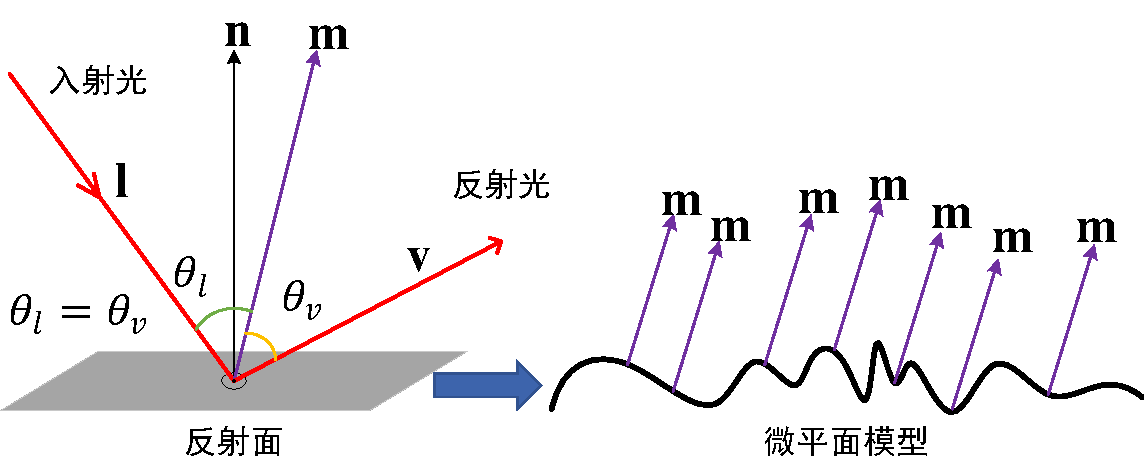
\includegraphics[width=0.8\linewidth]{FIG/Microfacetmodel.pdf}
  \caption{微平面模型}
  \label{fig:microfacet_model}
\end{figure*}
从几何光学的角度来说,大部分看似光滑的平面对于入射光的反射路径影响都非常大。从微观的角度将一个入射点看成是一个很小的区域,它由多个微小平面组成,其中只有以$\mathbf{m}$为法线的微平面可以将 $\mathbf{l}$ 方向射入的光反射到$\mathbf{v}$方向,如图\ref{fig:microfacet_model}所示。

\begin{figure*}[!t]
  \centering
  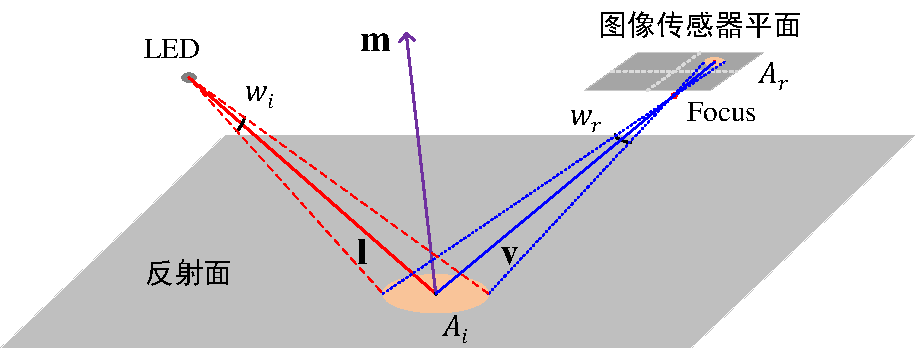
\includegraphics[width=0.8\linewidth]{FIG/reflected surface.pdf}
  \caption{反射成像过程}
  \label{fig:reflecting_image}
\end{figure*}
根据针孔相机模型,反射光$\mathbf{v}$将经过相机的焦点到达图像传感器某一个像素区域上,如图\ref{fig:reflecting_image}所示。为了计算图像传感器上任意一个点的亮度值,我们假设入射光束$\mathbf{l}$在立体角$w_{i}$内照射到反射面上以点$(x_{i},y_{i})$为中心的面积大小为$A_{i}$的区域上。 出射光束$\mathbf{v}$ 以立体角$w_{i}$经过相机的焦点照射到图像传感器上以点$(x_{r},y_{r})$为中心的面积大小为$A_{r}$的区域上。双向反射分布函数 BRDF 被定义为出射光的辐亮度和入射光的辐照度的比值随出射角度的方向分布,其公式为:
\begin{equation}\label{eq:fr}
  f_{r}=L_{r}/E_{i}
\end{equation}
已知:
\begin{equation}\label{eq:dei}
  E_{i}=\cos\theta_{i}L_{i}w_{i}
\end{equation}
其中,$L_{i}$是点$(x_{i},y_{i})$处的亮度,$\theta_{i}$是平面$A_{i}$的法线$\mathbf{l}$和$\mathbf{n}$的夹角。反射光的辐亮度可以表示为:
\begin{equation}\label{eq:dlrdphir}
  L_{r}=\Phi_{r}/w_{r}\cos\theta_{r}A_{r}
\end{equation}
与此同时,
\begin{equation}\label{eq:dArdAi}
  A_{i}=\delta A_{r}
\end{equation}
其中,$\Phi_{r}$是反射光在$A_{r}$区域上的辐射通量,$\theta_{r}$是$\mathbf{n}$和 $\mathbf{v}$的夹角。当图像传感器和LED的位置相对固定时,$\delta$是一个常数。注意,由于光通量的损失,反射的光通量可以由以下公式给出:
\begin{equation}\label{eq:dphirgf}
  \Phi_{r}=G(\mathbf{l},\mathbf{m},\mathbf{v})F(\mathbf{m},\mathbf{v})\Phi_{m}
\end{equation}
其中,$F(\mathbf{m},\mathbf{v})$是菲涅尔系数,它描述了法线方向为$\mathbf{m}$的微平面上的折射和反射分量的比率。几何衰减系数$G(\mathbf{l},\mathbf{m},\mathbf{v})$描述了相邻微平面分别在$\mathbf{l}$ 和 $\mathbf{v}$方向上的阴影和遮蔽效应。$\Phi_{m}$ 是在$A_{i}$区域上所有以$\mathbf{m}$为法线的微平面的发射通量之和,经过反射之后,其中的一部分反射通量$\Phi_{r}$在经过$G(\mathbf{l},\mathbf{m},\mathbf{v})$和 $F(\mathbf{m},\mathbf{v})$的衰减之后到达了图像传感器上。首先,$\Phi_{m}$可以表示为:
\begin{equation}\label{eq:dphim}
  \Phi_{m}=L_{i}w_{i}\cos\theta_{m}A_{m}
\end{equation}
在这里, $\theta_{m}$用来表示$\mathbf{m}$和 $\mathbf{l}$之间的夹角;$A_{m}$表示所有以$\mathbf{m}$为法线的微平面的面积之和,可以表示为:
\begin{equation}\label{eq:dAm}
A_{m}=D(\mathbf{m},\mathbf{n})w_{m}A_{i}
\end{equation}
在这里,$D(\mathbf{m},\mathbf{n})$是一个概率密度函数,用来表示以$\mathbf{m}$为法线的微平面相对于$A_{i}$区域上所有微平面的统计分布,是一个介于0和1之间的常数。



\begin{figure*}[!t]
\centering
  \begin{minipage}{0.45\linewidth}
    \centerline{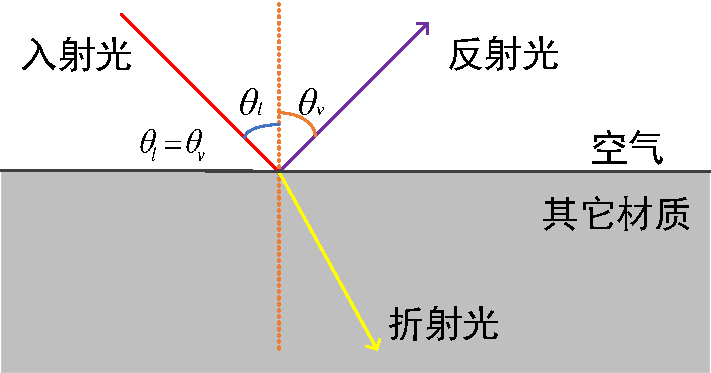
\includegraphics[width=\textwidth]{FIG/reflect process1.pdf}}
    \centerline{(a)}
  \end{minipage}
  \begin{minipage}{0.45\linewidth}
    \centerline{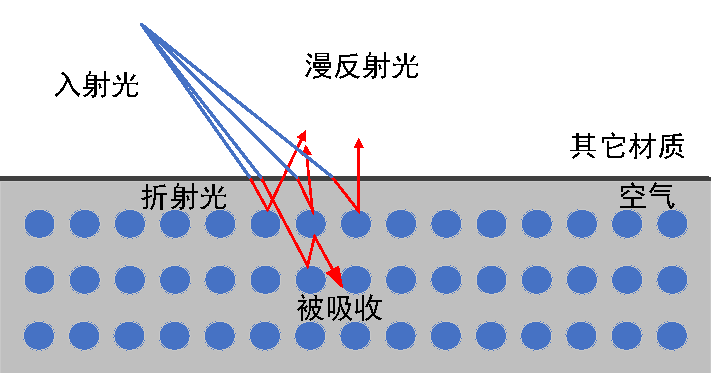
\includegraphics[width=\textwidth]{FIG/reflect process2.pdf}}
    \centerline{(b)}
  \end{minipage}\\
  \begin{minipage}{0.45\linewidth}
    \centerline{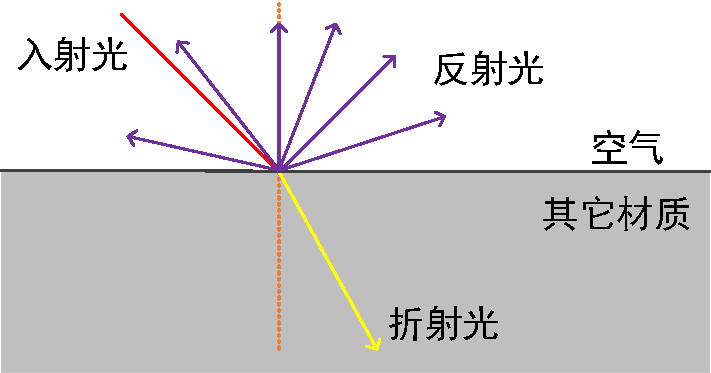
\includegraphics[width=\textwidth]{FIG/reflect process3.pdf}}
    \centerline{(c)}
  \end{minipage}
  \vfill
  \caption{(a) 入射光的反射和折射; (b) 漫反射的形成;(c)朗伯反射}
  \label{fig:Reflection and refraction}
\end{figure*}

将公式(\ref{eq:dei}), (\ref{eq:dlrdphir}), (\ref{eq:dArdAi}), (\ref{eq:dphirgf}), (\ref{eq:dphim}) 和 (\ref{eq:dAm})代入到公式 (\ref{eq:fr})中,有:
\begin{equation}\label{eq:frfdg0}
f_{r}=\frac{F(\mathbf{m},\mathbf{v})D(\mathbf{m},\mathbf{n})G(\mathbf{l},\mathbf{m},\mathbf{v})\cos\theta_{m}w_{m}\delta}{\cos\theta_{r}\cos\theta_{i}w_{r}}
\end{equation}
$D(\mathbf{m},\mathbf{n})$, $F(\mathbf{m},\mathbf{v})$以及$G(\mathbf{l},\mathbf{m},\mathbf{v})$ 分别可以表示为:
\begin{equation}\label{eq:Dm}
  D(\mathbf{m},\mathbf{n})=\frac{\partial^{2}}{\pi((\mathbf{n}\cdot\mathbf{m})^{2}(\partial^{2}-1)+1)^{2}}
\end{equation}
\begin{equation}\label{eq:Fm}
  F(\mathbf{m},\mathbf{v})=F_{0}+(1-F_{0})(1-(\mathbf{m}\cdot\mathbf{v}))^{5}
\end{equation}
\begin{equation}\label{eq:Glmv}
  G(\mathbf{l},\mathbf{m},\mathbf{v})=\frac{(\mathbf{n}\cdot\mathbf{v})}{(\mathbf{n}\cdot\mathbf{v})(1-k)}\frac{(\mathbf{n},\cdot\mathbf{l})}{k(\mathbf{n}\cdot\mathbf{l})(1-k)+k}
\end{equation}
其中,
\begin{subequations}\label{eq:akm}
  \begin{align}
  \partial&=r^{2} \label{eq:akmA}\\
  k&=(r+1)^{2}/8 \label{eq:akmB}\\
  \mathbf{m}&= (\mathbf{l}+\mathbf{v})/\left |\mathbf{l}+\mathbf{v}   \right | \label{eq:akmc}
  \end{align}
\end{subequations}
  
  $F_{0}$ 是入射角度为0时的菲涅尔系数; $r$ 是粗糙系数。
$w_{m}$和$w_{r}$之间存在这样的关系:
\begin{equation}\label{eq:dwmdwr}
w_{m}/w_{r}=1/4\cos\theta_{m}
\end{equation}
为了简化表达,在本文的余下部分,会分别用$F$, $D$ 和$G$来表示$F(\mathbf{m},\mathbf{v})$, $D(\mathbf{m},\mathbf{n})$以及$G(\mathbf{l},\mathbf{m})$。将公式(\ref{eq:dwmdwr})代入到公式 (\ref{eq:frfdg0})中,反射光的BRDF可以进一步表示为:
\begin{equation}\label{eq:frfdg1}
  f_{r}=\frac{\delta FDG}{4\cos\theta_{r}\cos\theta_{i}}
\end{equation}

根据几何光学理论,从一种介质入射到另一种介质的光会同时发生反射和折射,见图\ref{fig:Reflection and refraction}(a);一些折射的光会被吸收,而剩下的光会在材料内多次反射后以随机的方向从介质中出射,如图\ref{fig:Reflection and refraction}(b)所示。注意,漫反射是由于随机出射的光形成的,在这里被认为是朗伯反射,如图\ref{fig:Reflection and refraction}(c)所示。漫反射的BRDF由下面的公式给出:
\begin{equation}\label{eq:fd}
  f_{d}=c/\pi
\end{equation}
其中,$c$是一个常数,代表从反射面出射的光线(即那些没有被吸附的剩余光线)占总折射光线的比例。同时考虑镜面反射率和漫反射率的影响,BRDF的计算方法是:
\begin{equation}\label{eq:f}
  f=k_{d}f_{d}+k_{s}f_{r}=\frac{k_{d}c}{\pi}+\frac{k_{s}\delta FDG}{4\cos\theta_{r}\cos\theta_{i}}
\end{equation}
其中,$k_{s}$ 和 $k_{d}$分别是反射光和折射光的占比,如图\ref{fig:Reflection and refraction}(a)所示,它们之间的关系可以表示为:
\begin{equation}\label{eq:ks+kd=1}
  k_{s}+k_{d}=1
\end{equation}
基于公式(\ref{eq:It})和(\ref{eq:dei})发光强度和辐射强度之间的关系,$E_{i}$ 可以表示为:
\begin{equation}\label{eq:deicos}
  E_{i}=\cos\theta\cos\theta_{i}I_{N}(t)/d^{2}
\end{equation}
其中,$d$是 LED和$(x_{i},y_{i})$之间的距离。用公式(\ref{eq:f})中的$f$来代替公式(\ref{eq:fr})中的$f_{r}$,有:
\begin{equation}\label{eq:dLr-last}
  L_{r}=\frac{\cos\theta\cos\theta_{i}I_{N}(t)}{d^{2}}(\frac{k_{d}c}{\pi}+\frac{k_{s}\delta FDG}{4\cos\theta_{r}\cos\theta_{i}})
\end{equation}

除了光源的直接照射外,来自墙壁的多次反射的照射将被视为背景噪音。在每个反射过程中也会发生折射和反射,折射的部分会被部分吸收,从而导致能量的损失。在这里,本文暂不考虑这部分光所形成的亮度。

本系统最终关注的是每个像素的光亮度,用$\Omega_{p}$来表示像素$(u,v)$所在区域,其亮度为$L_{r}$。显然,可以用一个常数 $\Omega_{0}$来表示$\Omega_{p}$区域的面积。实际上,在整张图片曝光过度过程中,相机和LED的位置是固定的,$\mathbf{n}$表示反射面宏观上的法线。根据针孔相机模型,点$(x_{i},y_{i})$可以由点$(x_{r},y_{r})$来确定。因此,$\mathbf{l}$,$\mathbf{m}$, $\mathbf{v}$, $\theta_{r}$, $\theta_{i}$以及 $L_{r}$ 都可以表示成$(x_{r},y_{r})$的函数,有:
  \begin{equation}\label{eq:Lruvt}
    L_{r}(u,v,t)= \iint\limits_{\Omega_{p}}^{}L_{r}(x_{r},y_{r},t)/\Omega_{0}d\Omega
  \end{equation}
考虑到只有$I_{N}(t)$与时间有关,因此,亮度$L_{r}(u,v,t)$可以分解成为时间和空间两个分量:
  \begin{equation}\label{eq:LruvtINtLr}
    L_{r}(u,v,t)= I_{N}(t)L_{r}(u,v)
  \end{equation}
其中,时间分量可以表示为: 
  \begin{equation}\label{eq:Lruv}
    L_{r}(u,v)= \frac{\cos\theta\cos\theta_{i}}{d^{2}\Omega_{0}}\iint\limits_{\Omega_{p}}^{}(\frac{k_{d}c}{\pi}+\frac{k_{s}\delta FDG}{4\cos\theta_{r}\cos\theta_{i}})d\Omega
  \end{equation}
现在,可以知道公式\ref{eq:LruvtINtLr}表示的是在时间t像素$(u, v)$区域内的平均亮度,这也是本文所提出的亮度分布模型 (LDM)。

\begin{figure*}[!t]
  \centering
  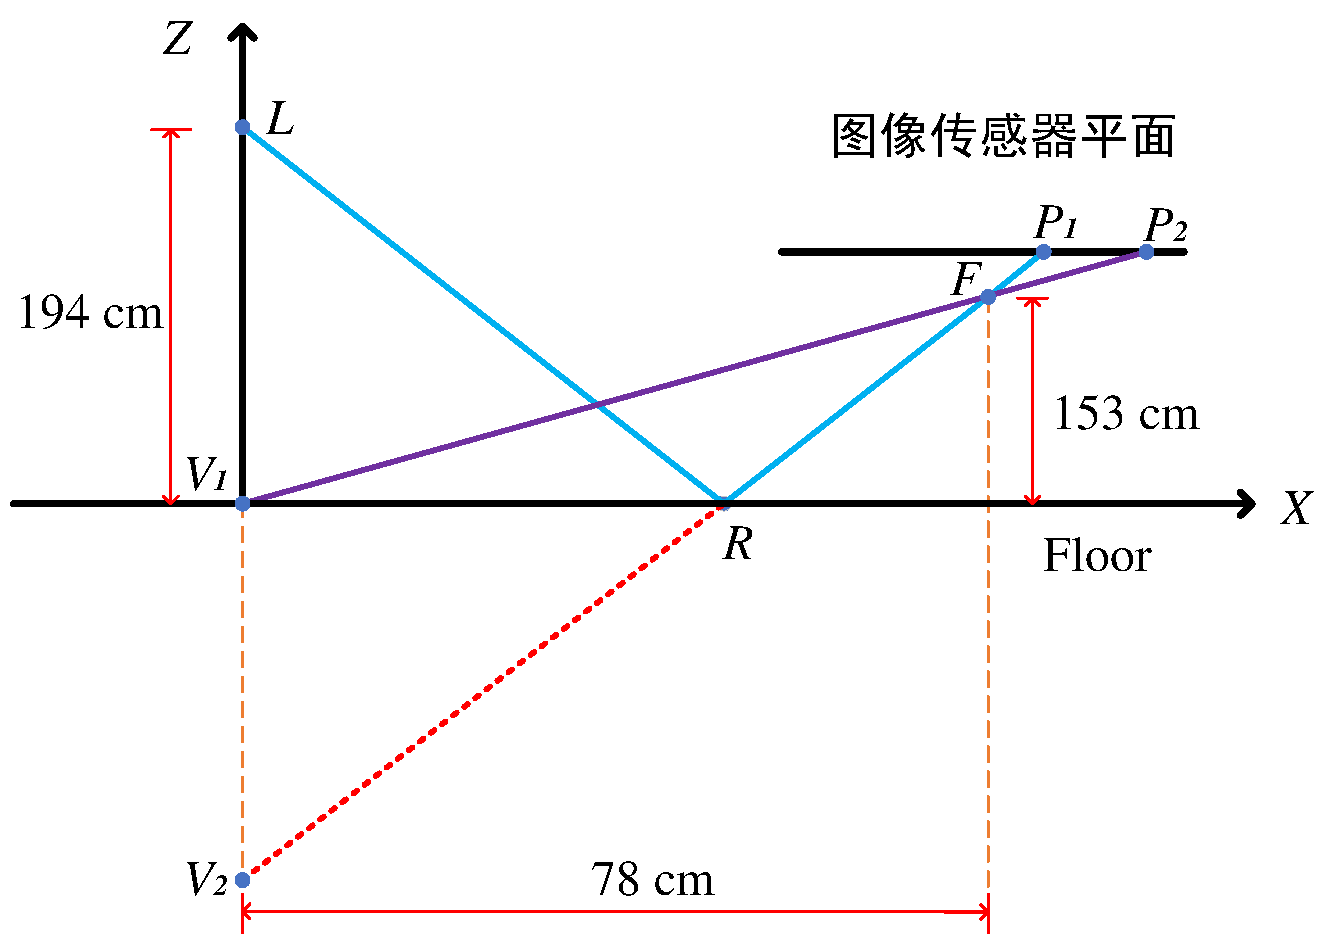
\includegraphics[width=0.6\linewidth]{FIG/simulationenvironment.pdf}
  \caption{几何仿真参数}
  \label{fig:simulate_data}
\end{figure*}
为了对LDM进行仿真,做以下假设:
\begin{enumerate}[topsep = 0 pt, itemsep= 0 pt, parsep=0pt, partopsep=0pt, leftmargin=20pt, itemindent=0pt, labelsep=6pt, label={(\arabic*)}] 
    \item{LED和IS表面与地板平行。将LED在地板上的投影点视为坐标原点,将相机焦点在地板上的投影点与原点之间的连线视为$x$轴,$z$轴与之垂直,并且确保IS平面的长边与$x$轴平行。}
    \item{LED的发射功率维持不变,即 $I_{N}(t)=I_{0}$,因此$L_{r}(u,v,t)$与时间无关。}
  \end{enumerate} 
  
  
简单的仿真几何模型如图\ref{fig:simulate_data}所示,其中$L$表示LED的位置,$V_{1}$是点$L$在地板上的投影,$V_{2}$是$L$关于地板的对称点,$F$表示相机的焦点,而$V_{1}F$和$V_{2}F$分别在$P_{1}$和$P_{2}$处与图像传感器平面相交。
使用表\ref{tab:parameters of simulation}中的参数对LDM进行仿真。 
 \begin{table}[!b]
                \centering  
                \caption{亮度分布模型的仿真参数}  
    \label{tab:parameters of simulation} 
                \begin{tabular}{lc}  
                \toprule
                \makebox[0.35\linewidth][l]{$\textbf{仿真参数}$} &\makebox[0.5\linewidth][c]{$\textbf{参数值}$}\\ 
                  \midrule  
                  $\mathbf{L}$坐标 & (0, 0, 194) cm \\
      $\mathbf{V_{1}}$坐标 & (0, 0, 0) \\ 
      $\mathbf{V_{2}}$坐标 & (0, 0, -194) cm \\ 
      $\mathbf{F}$ 坐标& (78, 0, 153) cm  \\
      菲涅尔系数$F_{0}$ &  0.04\\
      折射系数$k_{s}$ &  0.7\\
      出射系数$c$ & 0.9\\
      粗糙系数$r$ & 0.01\\
      LED发光强度$I_{0}$ & 1000 cd\\
                  \bottomrule 
                \end{tabular}
    \end{table}





仿真结果如图\ref{fig:simulate_result}所示,其中在坐标为(0.890,0.001)和(2.050,0.002) mm处检测到两个极值点,即$M_{1}$和$M_{2}$,这表示通过系统的仿真结果,可以知道当只有一个LED发光的时候,通过对反射面进行成像的照片上可以捕捉到两个光斑,这与实际的观察结果相同。

\begin{figure*}[!t]
  \centering
  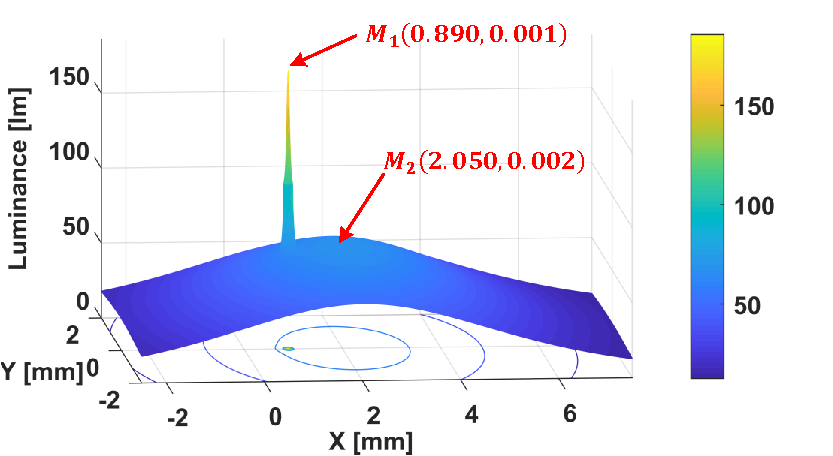
\includegraphics[width=0.8\linewidth]{FIG/BRDF.pdf}
  \caption{亮度分布模型的仿真结果}
  \label{fig:simulate_result}
\end{figure*}
根据针孔相机模型,已知$P_{1}$和$P_{2}$分别是$V_{1}$和$V_{2}$在图像传感器上的投影。因此,$P_{1}$和$P_{2}$的坐标通过计算可以得到,分别是(0.897,0)和(2.034,0) mm,这与$M_{1}$和$M_{2}$的坐标基本上一致。

如果将$V_{1}$和$V_{2}$看作是两个虚拟LED,我们根据$P_{1}$、$P_{2}$和$M_{1}$、$M_{2}$之间位置关系的一致性可以得出如下结论:在对反射面进行成像的过程中,就高光点在图像上的位置来说,$L$的效果与两个虚拟LED $V_{1}$和$V_{2}$的效果基本上相同。换言之,捕获的图像中的两个高光点可以被视为两个虚拟LED通过LOS路径形成的投影,其中一个是LED关于地板的对称点,另一个是LED在地板上的投影。




\section{系统流程}
通过LDM的结论可以知道,在只有一个LED发光的时候,反射面的图像上可以检测到两个高光点,并且两个高光点的位置可以看成是两个虚拟LED通过LOS路径形成的投影,其中一个是LED关于地板的对称点,另一个是LED在地板上的投影。由此,本系统的所设计的基于单点定位算法的NLOS IS-VLP实际上可以转换成基于两个虚拟的LED的LOS IS-VLP。因此,本系统具体的定位算法采用了前面所述的重投影误差最小化,将两个虚拟的LED世界坐标和两个高光点的像素坐标代入公式(\ref{mx:reprojection})即可得出最终的相机位置。需要注意的是,本系统并不能实现任意姿态的3D定位,需要图像传感器平面平行于地面,此时旋转矩阵$\mathbf{R}$只跟一个角度有关,通过地面的标记很容易测量出这个角度。

本系统的简化模型如图\ref{fig:firstsystemmodel}所示,整个系统主要由三个部分组成:虚拟LED坐标的获取、高光亮点的几何提取和最终的位置估计。
\begin{figure*}[!t]
  \centering
  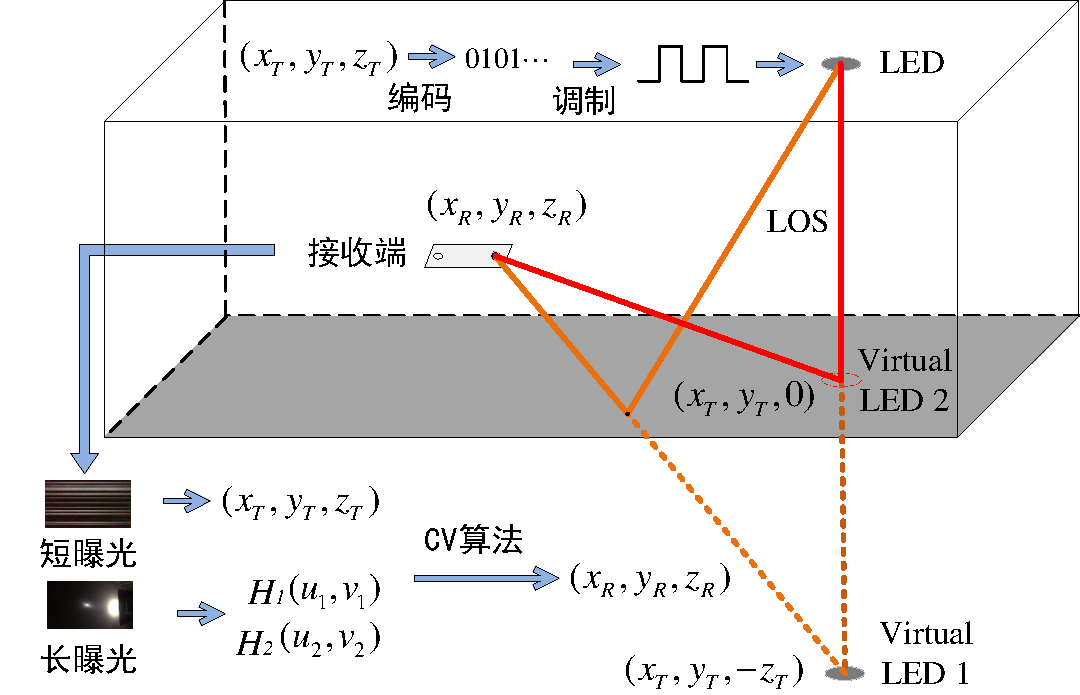
\includegraphics[width=0.7\linewidth]{FIG/First systemmodel.pdf}
  \caption{系统模型}
  \label{fig:firstsystemmodel}
\end{figure*}


首先是虚拟LED坐标的获取,通过第三章的NLOS OCC系统,可以获得LED坐标$(x_T,y_T,z_T)$。由前面所述的LED与两个虚拟LED之间的位置关系,两个虚拟LED的坐标$V_1(x_{v1},y_{v1},z_{v1})$和$V_2(x_{v2},y_{v2},z_{v2})$可以表示为:
 \begin{equation}\label{v1v2}
    \begin{cases} 
              x_{v1}=x_{v2}=x_{T} \\
              y_{v1}=y_{v2}=y_{T}   \\     
              z_{v1}=-z_{T}\\
              z_{v2}=0             
    \end{cases}
\end{equation}
        
 \begin{figure}[!htbp]
    \centering
              \begin{minipage}{0.3\linewidth}
                \centering
                \centerline{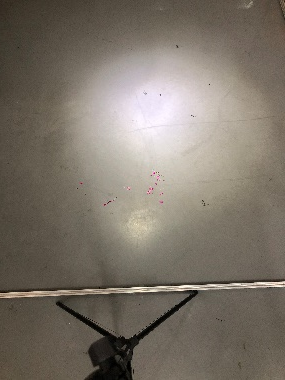
\includegraphics[width=\textwidth]{FIG/fig9(a).png}}
                \centerline{(a)}
              \end{minipage}
              \begin{minipage}{0.3\linewidth}
                \centering
                \centerline{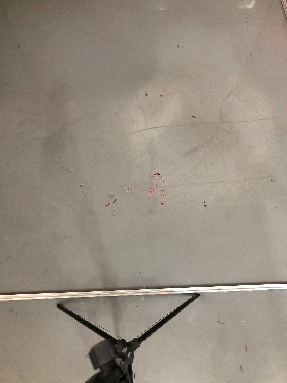
\includegraphics[width=\textwidth]{FIG/fig9(b).png}}
                \centerline{(b)}
              \end{minipage}\\
              \begin{minipage}{0.3\linewidth}
                \centering
                \centerline{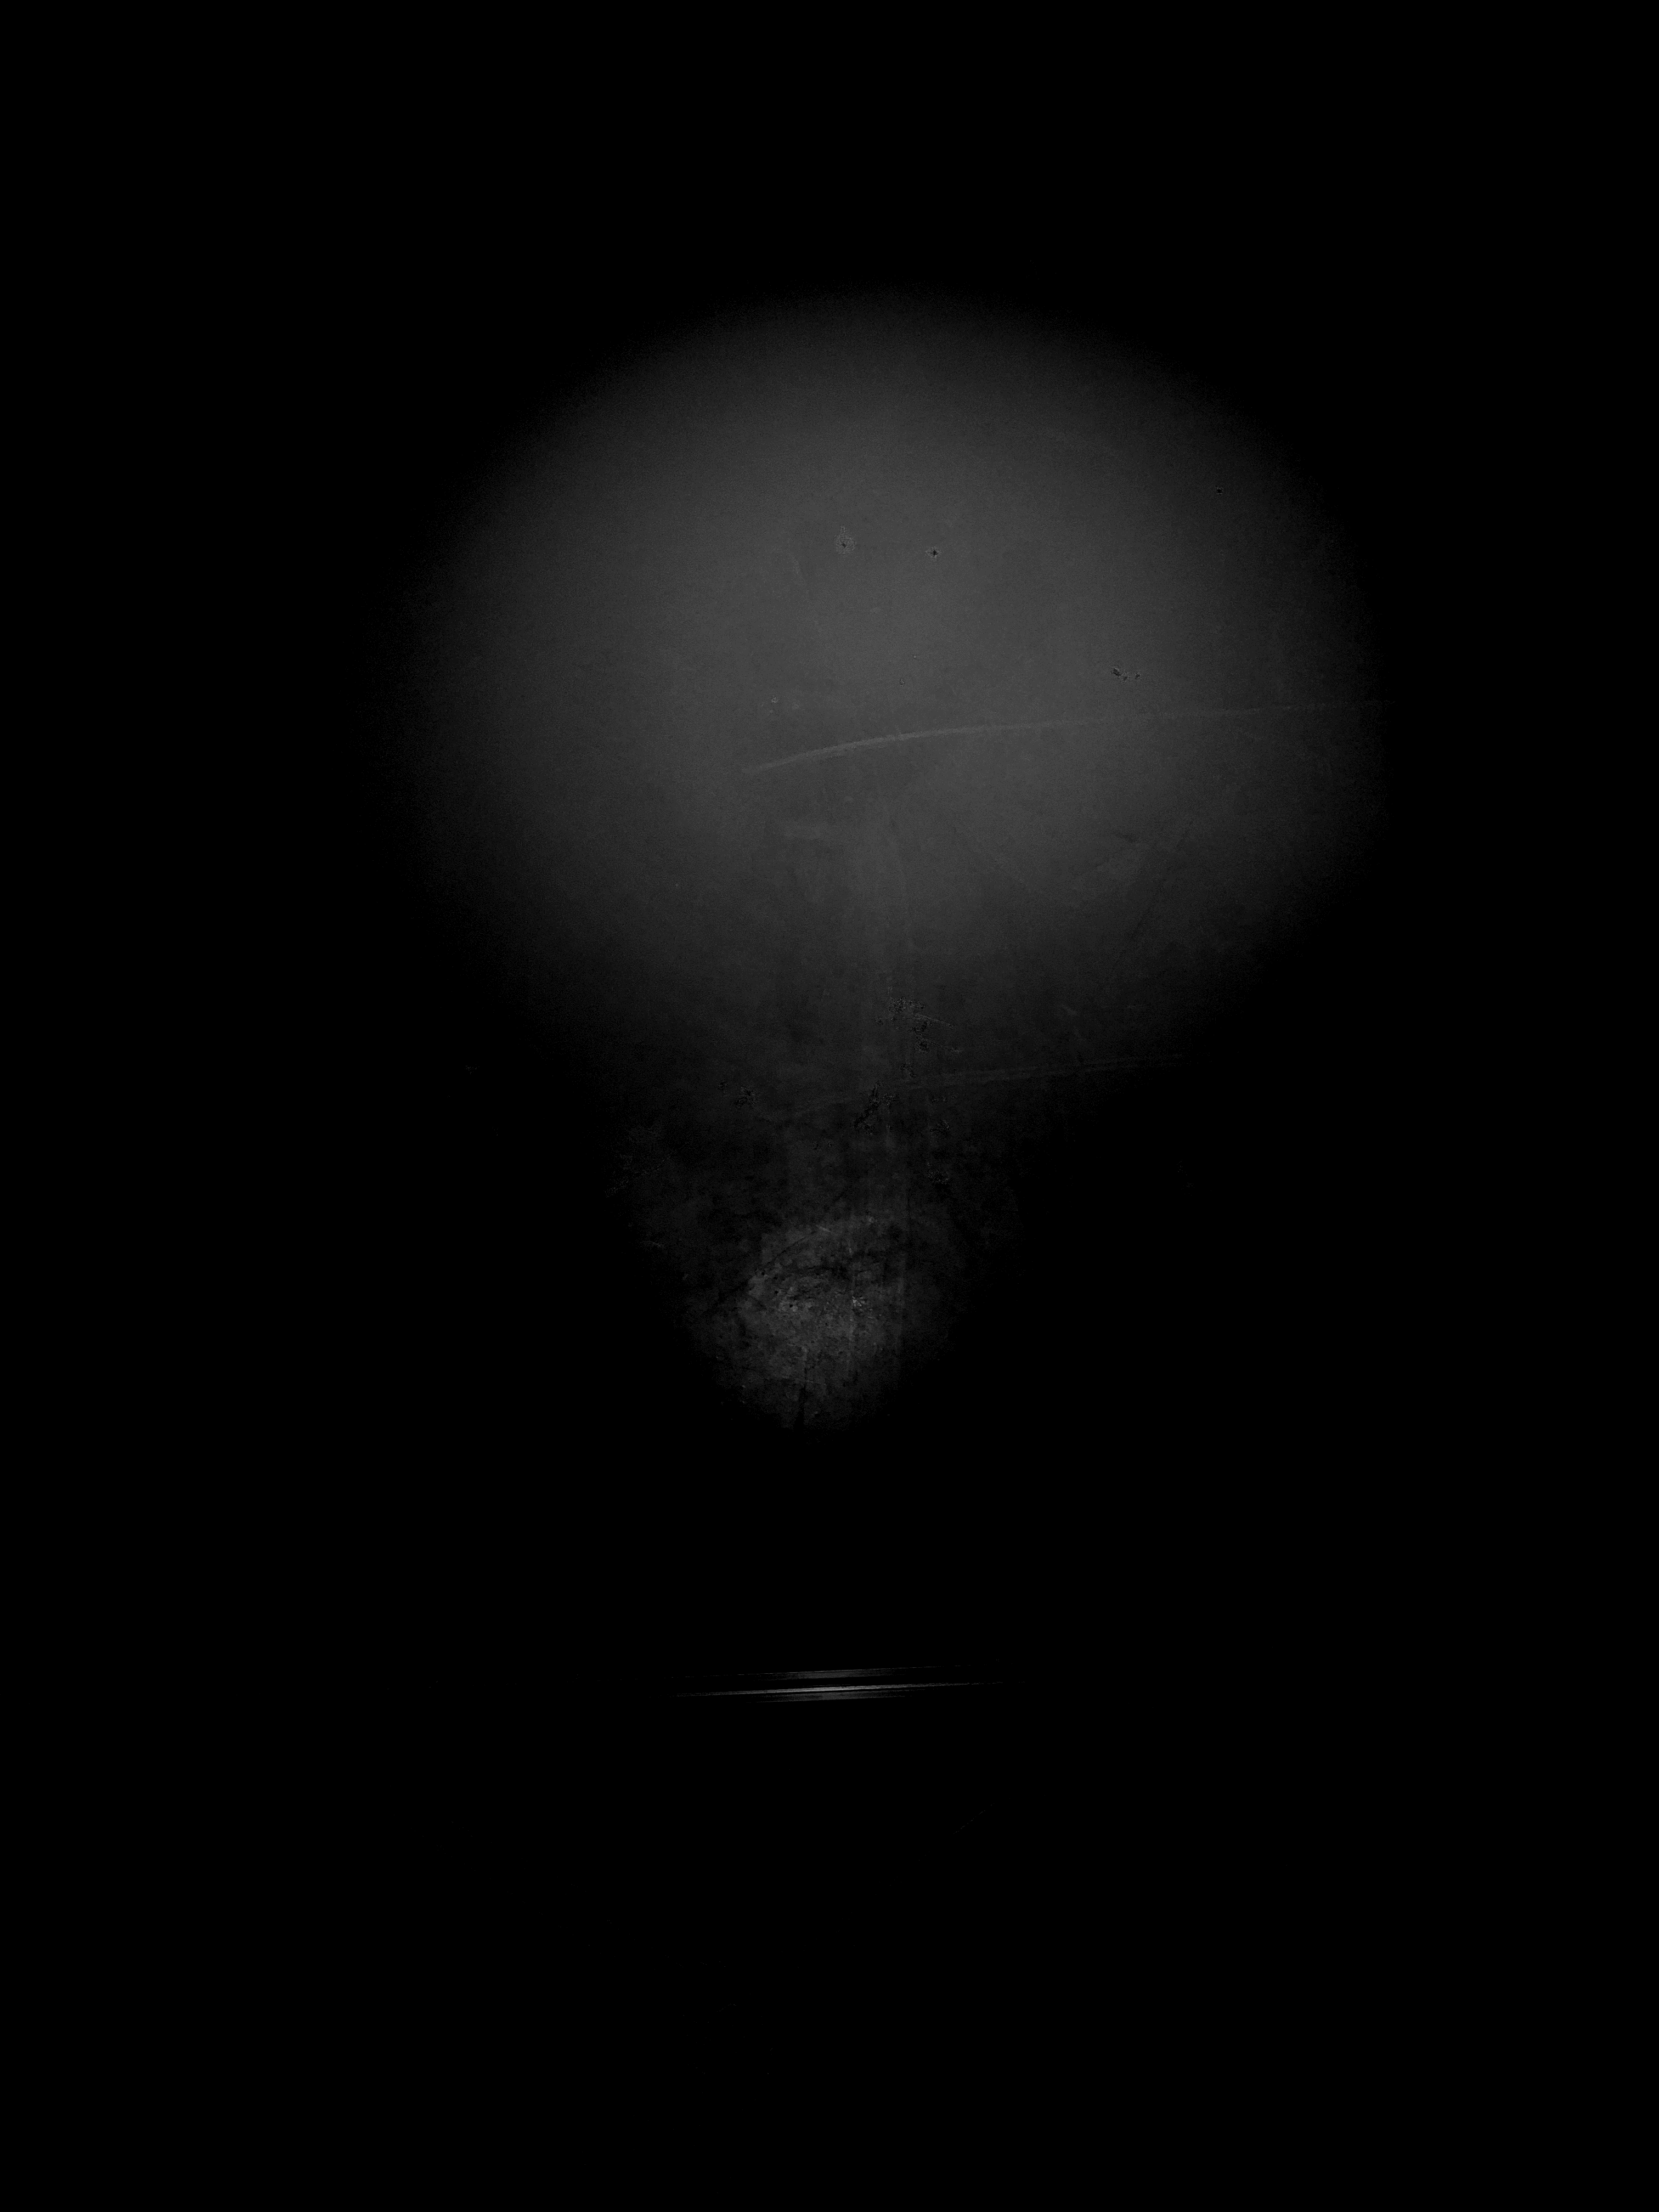
\includegraphics[width=\textwidth]{FIG/fig9(c).png}}
                \centerline{(c)}
              \end{minipage}
              \begin{minipage}{0.3\linewidth}
                \centering
                \centerline{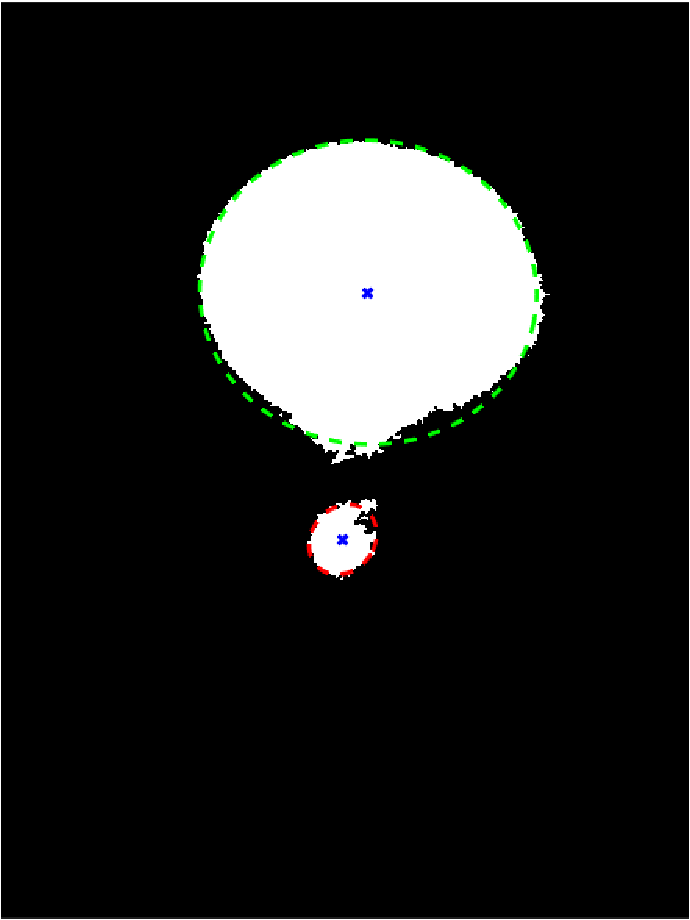
\includegraphics[width=\textwidth]{FIG/fig9d.pdf}}
                \centerline{(d)}
              \end{minipage}
              \vfill
              \caption{两个高光坐标提取:(a) 前景; (b)背景; (c) 降噪;(d) 椭圆拟合}
              \label{fig:image processing}
  \end{figure}

使用边缘检测和椭圆拟合提取两个高光的位置,分别是$H_1(u_1,v_1)$和$H_2(u_2,v_2)$。如图\ref{fig:image processing}(a)和图\ref{fig:image processing}(b)所示,当LED打开和关闭时,分别拍摄了两张反射面的照片。如图\ref{fig:image processing}(c)所示,可以使用帧减法和频域滤波来减少背景光引起的干扰。两个亮点周围的区域,在阈值滤波之后通过检测两个最大的连通域得到。接下来,检测两个高光的边缘,并用椭圆曲线拟合,如图\ref{fig:image processing}(d)所示。在每一级阈值滤波之后,将连接域中的像素数作为权重因子,并通过对每个椭圆拟合曲线的中心坐标进行加权平均来获得两个亮点的最终坐标,其由下式给出:
 \begin{equation}\label{highlightspixel}
              \begin{cases} 
                (u_{1},v_{1})=\sum_{i=1}^{m}\frac{a_{1}(i)}{n_{1}}(u_{1i},v_{1i})   \\
                (u_{2},v_{2})=\sum_{i=1}^{m}\frac{a_{2}(i)}{n_{2}}(u_{2i},v_{2i})              
              \end{cases}
\end{equation}
其中$a_{1}(i)$和$a_{2}(i)$表示$S_1$和$S_2$在第$i$级阈值下的连通域像素数,$(u_{1i},v_{1i})$和$(u_{2i},v_{2i})$表示其坐标,而$n_{1}$和$n_{2}$表示$S_1$和$S_2$在所有$m$级阈值下的连通域像素的总数,$m$由灰度值的直方图决定。

将两个虚拟的LED世界坐标和两个高光点的像素坐标以及测量的$\mathbf{R}$代入公式(\ref{mx:reprojection}),通过重投影误差最小化算法即可得出最终的相机位置。

\section{实验与性能}
\subsection{实验环境}
首先,发射端LED固定于距离地面1.96 m的高度,iPhone 8的后摄被用于接收端。手机连接在一个带有水平仪的支架上,调整支架使其平行于地面。将地面测试区域划分为5 $\times$ 5的方格,每个网格的边长为0.3m,LED在网格中间点的正上方。通过移动支架的位置来收集24个网格顶点的数据,并测试系统在这24个网格顶点位置的定位精度。本文会采用黑布将实验区域遮住来测试有无环境光和多次反射对实验结果的影响。硬件系统由工作频率为3.3 kHz的STM32微控制器单元、直流电源以及LED等组成,如图\ref{fig:Fir_setup}所示。表\ref{tab:Fir_experiments parameters}中给出了所有关键的系统参数。
 \begin{figure}[!htbp]
                \centering
                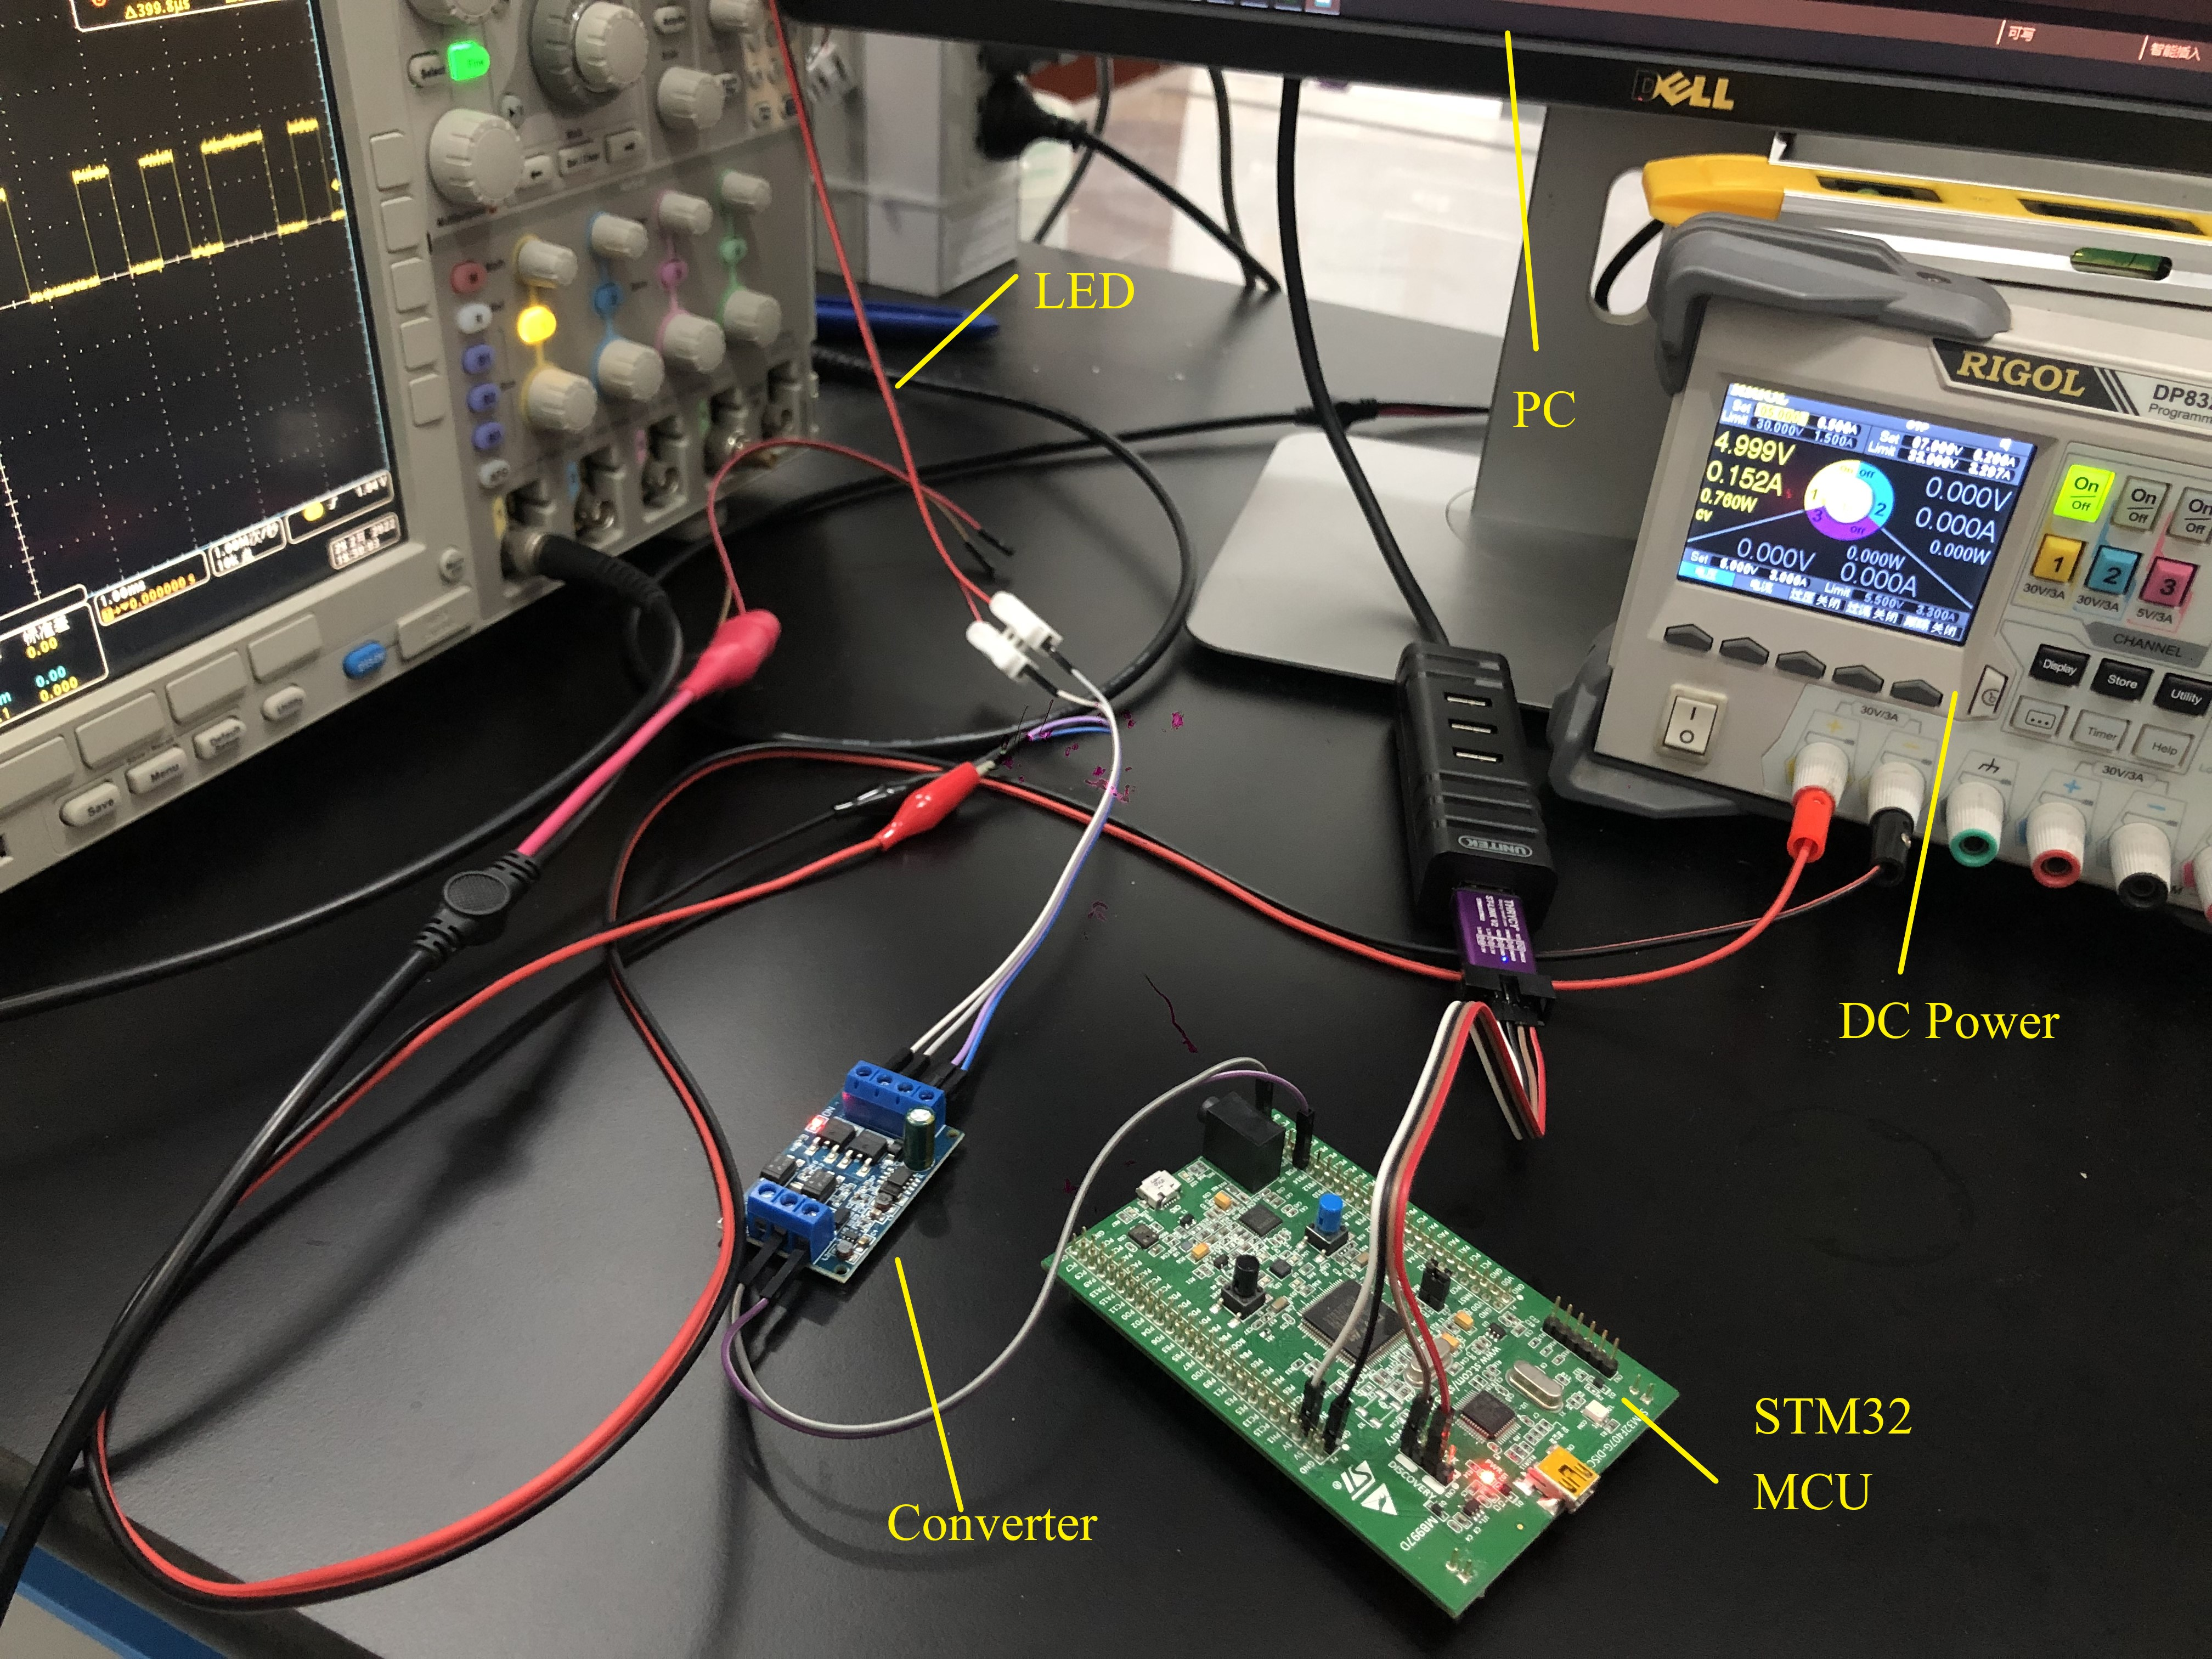
\includegraphics[width=0.6\linewidth]{FIG/fig10-hardware.jpg}
                \caption{系统测试硬件平台}
                 \label{fig:Fir_setup}
\end{figure}
 \begin{table}[!htbp]
                \centering  
                \caption{基于亮度分布模型的NLOS VLP系统实验参数}  
                \label{tab:Fir_experiments parameters}  
                \begin{tabular}{lc}  
                \toprule
                \makebox[0.35\linewidth][l]{$\textbf{实验参数}$} &\makebox[0.5\linewidth][c]{$\textbf{参数值}$}\\ 
                  \midrule  
                  测试环境 & 1.84 $\times$ 1.84 $\times$ 1.96 $\mathrm{m^{3}}$   \\ 
                  LED 输出功率 & 5 $\mathrm{W}$  \\
                  LED 坐标 &  (0, 0, 1.96) $\mathrm{m}$\\
                  LED 工作电压范围 & 3-5 $\mathrm{V}$\\
                  MCU 输出频率 & 3.3 $\mathrm{kHz}$\\
                  相机焦距 & 3.99 $\mathrm{mm}$\\
                  像素面积 & 1.19 $\times$ 1.19 $\mathrm{\mu m^{2}}$\\
                  像素尺寸 & 4032 $\times$ 3024\\
                  \bottomrule 
                \end{tabular}
    \end{table}
    
\subsection{系统性能}

本系统通过测试放置在5 $\times$ 5网格顶点上的智能手机的位置来评估所提出的NLOS IS-VLP系统的3D定位性能。本系统分别在131 cm和153 cm高度下对有无环境光的场景进行了测试,对这三种情况都计算了24组数据的均方根误差(Root Mean Squared Error, RMSE)和的平均定位误差。实验结果如表\ref{tab:results-average}所示,其中无环境光时最低的平均误差和RMSE分别为15.9和16.8 cm。然而,将高度从131 cm增加到153 cm会导致平均误差和RMSE都增加5个百分点左右。此时,在有环境光的条件下,平均误差和RMSE增加到19.65和22.50 cm。

此外,本系统还分别计算了不同情况下每个轴的平均误差,结果如表\ref{tab:results-average}所示。智能手机的高度为131 cm无环境光时X、Y和Z轴的最佳值分别为7.03、8.32和9.90 cm。将高度增加到153 cm,X、Y和Z轴的平均误差分别为5.84、7.80和11.31 cm。在有环境光的情况下,X、Y和Z轴上的平均误差值分别为5.92、6.92和15.56 cm。可以看出,距离和环境光干扰对系统性能的影响主要在Z轴上。 如图\ref{fig:errors-2D}所示,系统比较了有无环境光以及智能手机高度对X和Y轴定位精度的影响。注意,除了离中心点最远的几个测试点的位置外,其他所有位置在三种情况下都显示出良好的性能。在X-Y平面上,三种方案的2D误差没有明显差异。对于3D性能,几种情况差异增大,特别是在有环境光下将手机高度提高到153 cm,会导致Z轴上定位误差增大,如图\ref{fig:errors-3D}所示。
     \begin{table}[!t]
                \centering  
                \caption{NLOS IS-VLP系统定位性能}  
                \label{tab:results-average}  
                \begin{tabular}{lccccc}  
                  \toprule 
                \makebox[0.15\linewidth][l]{$\textbf{测试条件}$} &\makebox[0.1\linewidth][c]{$\textbf{X (cm)}$}&\makebox[0.1\linewidth][c]{$\textbf{Y (cm)}$}&\makebox[0.1\linewidth][c]{$\textbf{Z (cm)}$}&\makebox[0.2\linewidth][c]{$\textbf{平均误差 (cm)}$}&\makebox[0.15\linewidth][c]{$\textbf{RMSE (cm)}$}\\ 
                \midrule  
                  131 cm 遮光 & 7.03&8.32&9.90& 15.90&16.77  \\
                  153 cm 遮光& 5.84&7.80&11.31 & 16.68&17.63  \\
                  153 cm 无遮光 & 5.92&6.92&15.56& 19.65&22.50  \\
                  \bottomrule 
                \end{tabular}
\end{table}

  
     \begin{figure}[!htbp]
                \centering
                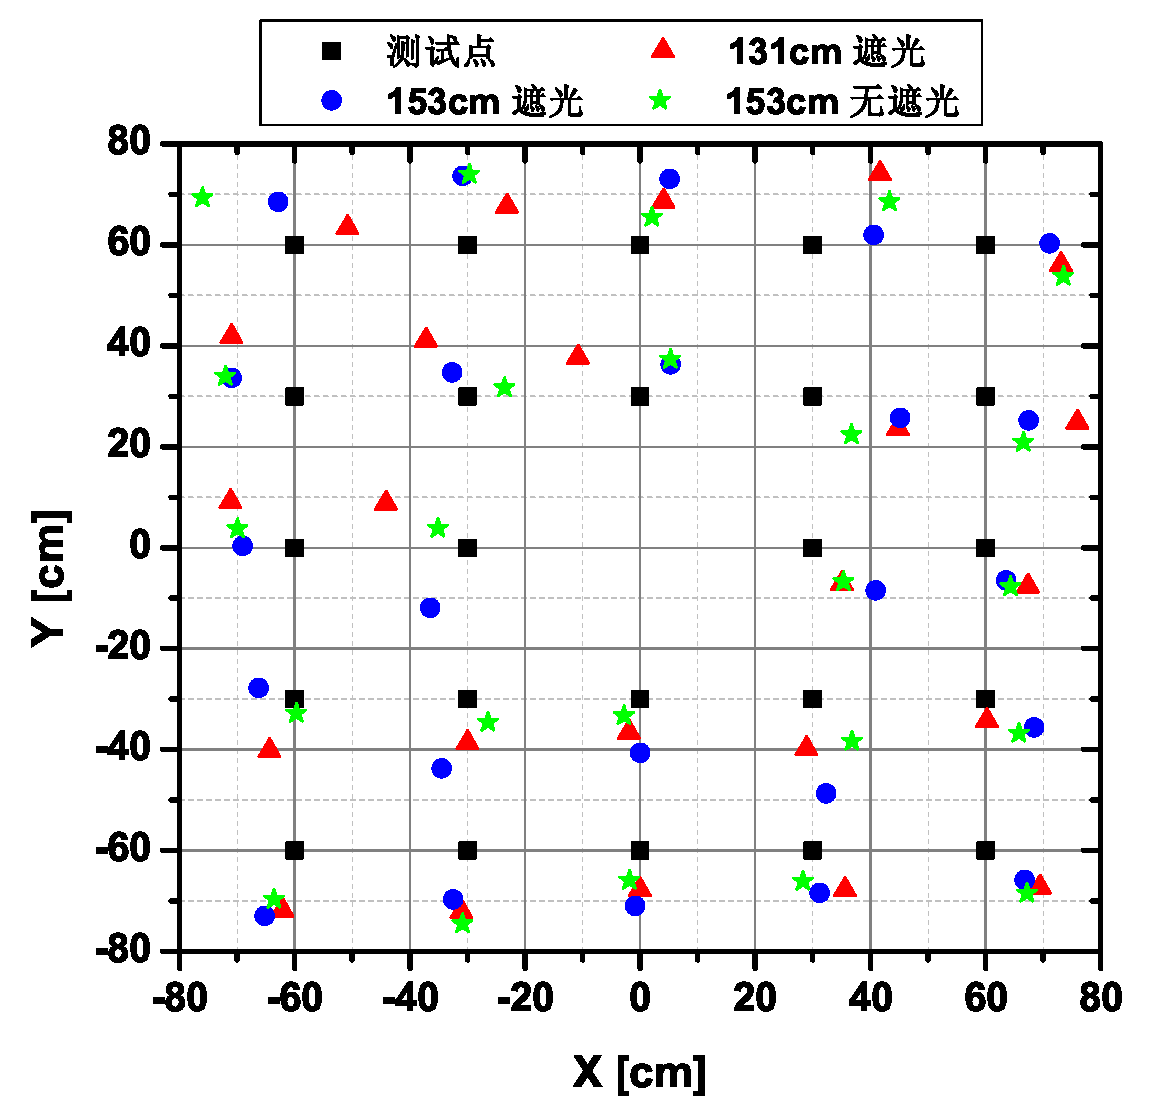
\includegraphics[width=0.7\linewidth]{FIG/5-8.eps}
                \caption{不同环境下的NLOS VLP系统2D性能}
                \label{fig:errors-2D}
\end{figure}


     \begin{figure}[!t]
                \centering
                \begin{minipage}{0.45\linewidth}
                  \centering
                  \centerline{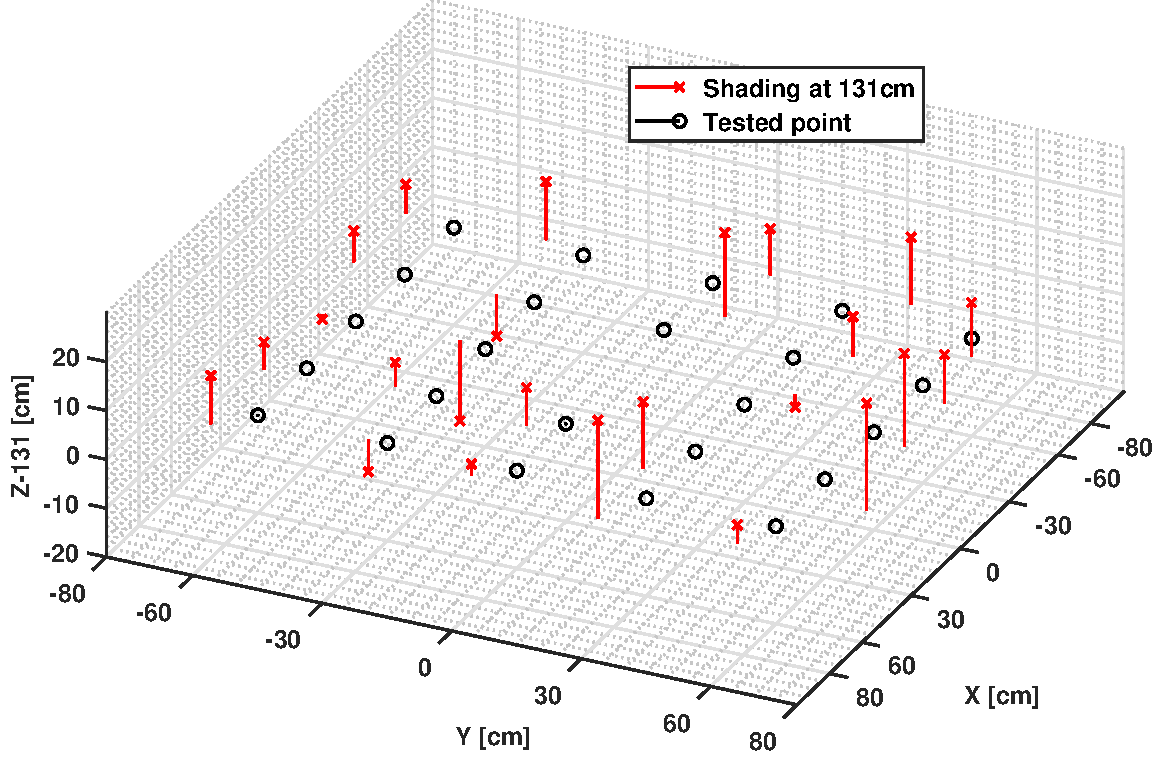
\includegraphics[width=\textwidth]{FIG/fig12a.pdf}}
                  \centerline{(a)}
                \end{minipage}
                \begin{minipage}{0.45\linewidth}
                  \centering
                  \centerline{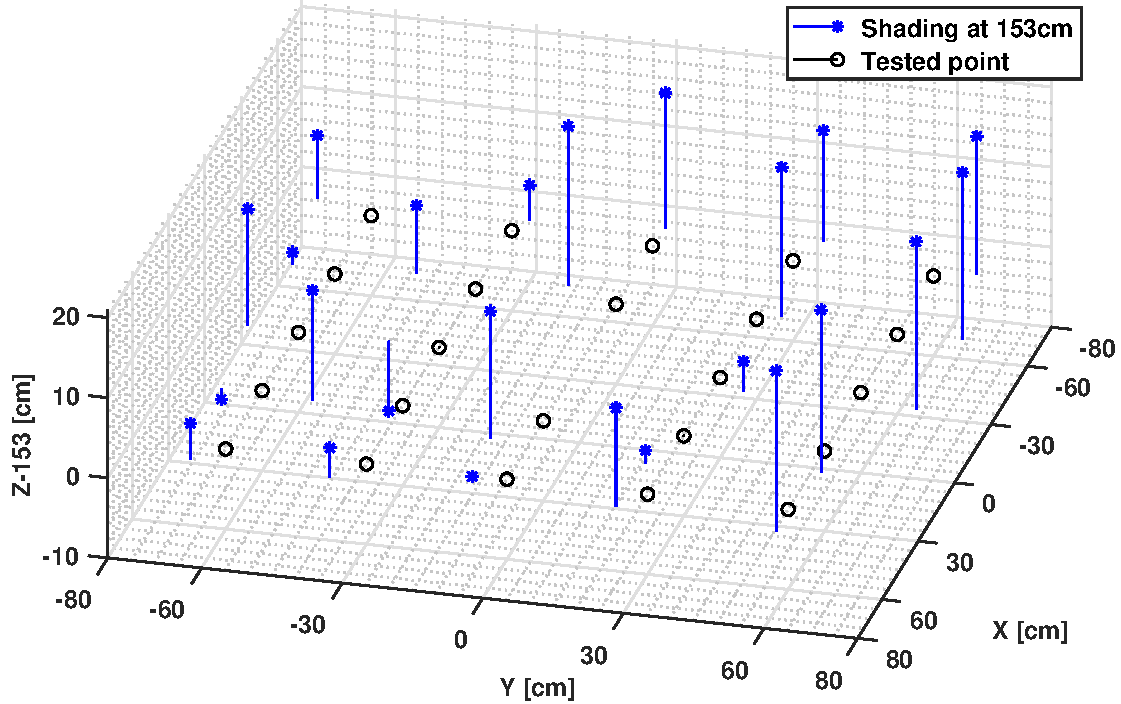
\includegraphics[width=\textwidth]{FIG/fig12b.pdf}}
                  \centerline{(b)}
                \end{minipage}\\
                \begin{minipage}{0.5\linewidth}
                  \centering
                  \centerline{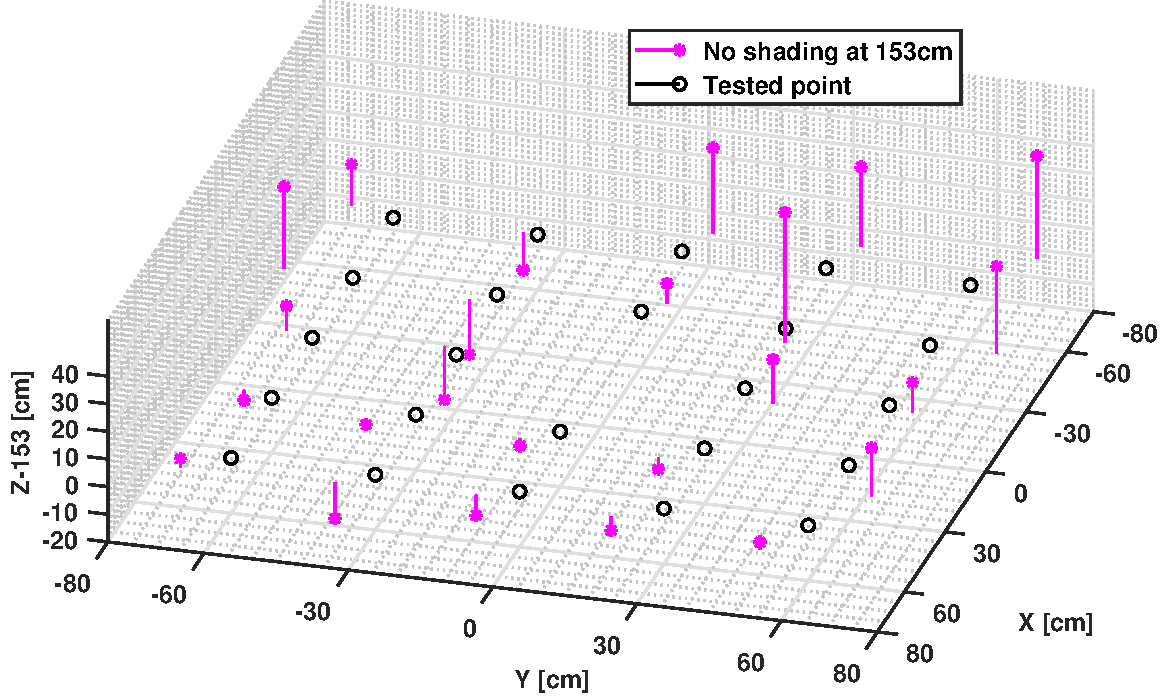
\includegraphics[width=\textwidth]{FIG/fig12c.pdf}}
                  \centerline{(c)}
                \end{minipage}
                \vfill
                \caption{NLOS VLP的3D定位性能: (a) 131 cm遮光; (b) 153 cm遮光; (c) 153 cm有环境光.}
                \label{fig:errors-3D}
 \end{figure}

因此,本系统分析了实验结果中的误差。在方程组(\ref{mx:world-ccww})中,由于$\mathbf{R}$实际上是已知的,为了忽略$\mathbf{R}$的影响,假设$\mathbf{R}$是单位矩阵,这样目标向量$-\mathbf{R}^{-1} \mathbf{t} $的误差分析就可以转化为$\mathbf{t}$的分析,现在,$(x_w,y_w,z_w )^T$是已知的。因此,改变$\mathbf{t}$与改变$(x_c,y_c,z_c)$是等价的。因此,将方程(\ref{mx:cemara-xycc})的左右两边都除以$z_c$并代入方程(\ref{mx:pixel-uvxy})中,并经过变形,得到:
    \begin{equation}\label{eq:u-u0}
                \frac{f_{0}x_{c}}{z_{c}}=\frac{f_{0}x_{c}}{z_{c}^{'}+\Delta z_{c}}=u-u_{0}=u^{'}+\Delta u-u_{0},
    \end{equation}
其中 $f_0=f/dx$,$\Delta u$ 是 $u$ 的估计误差,$\Delta z_c$ 是 $z_c$ 的估计误差,它是 函数(\ref{mx:world-ccww}) 和 (\ref{mx:reprojection}) 中的一个独立变量,因此 $x_c$ 将被视为 $z_c$ 的隐函数,而观察到的误差是由于 $z_c$引起的。公式(\ref{eq:u-u0}) 是一个理想的情况,而实际的计算过程如下:
     \begin{equation}\label{eq:u'-u0}
                \frac{f_{0}x_{c}}{z_{c}^{'}}=u^{'}-u_{0}.
  \end{equation}
 现在假设:
     \begin{equation}\label{eq:delta u}
        \Delta u= \eta (u^{'}-u_{0}),
    \end{equation}   
$\Delta z_{c}$可以表示为:
     \begin{equation}\label{eq:delta zc}
    \Delta z_{c}=\eta z_{c}.
\end{equation}
在实验中,$z_{c}=153$,所以,$\Delta z_c=153 \eta$。如果 $x_c$ 被视为函数(\ref{mx:world-ccww}) 和 (\ref{mx:reprojection}) 中的一个独立变量,那么 $z_c$ 可以被视为 $x_c$ 的隐函数。$x_c$ 的估计误差的最大值是 $ \Delta x_c \approx60 \eta$。相同的 $u$ 误差对 $x_c$ 和 $z_c$ 有完全不同的影响,因此也对 $y_c$ 有影响。另外,$\eta \approx 1$ 或者甚至 $\eta>1$ 可能对 $(u-u_0)\propto 0$ 成立,这会使得 $ \Delta z_c$ 倍增。换句话说,当手机放置在LED正下方时,将观察到最大的定位误差。这就是不计算中心点误差的原因。在这种情况下,当高亮点接近图像中心时,相机位置被认为是直接在LED下方。另外,在仔细分析图 \ref{fig:errors-3D} 中的误差分布时,可以观察到最大的误差集中在第二象限,这里靠近窗户,室外直射光对这个区域有很大的影响。通过图 \ref{fig:errors-3D}可以得出结论:环境光引起的干扰比传输距离对z轴定位精度的影响更严重。

 \begin{figure}[!t]
                \centering
                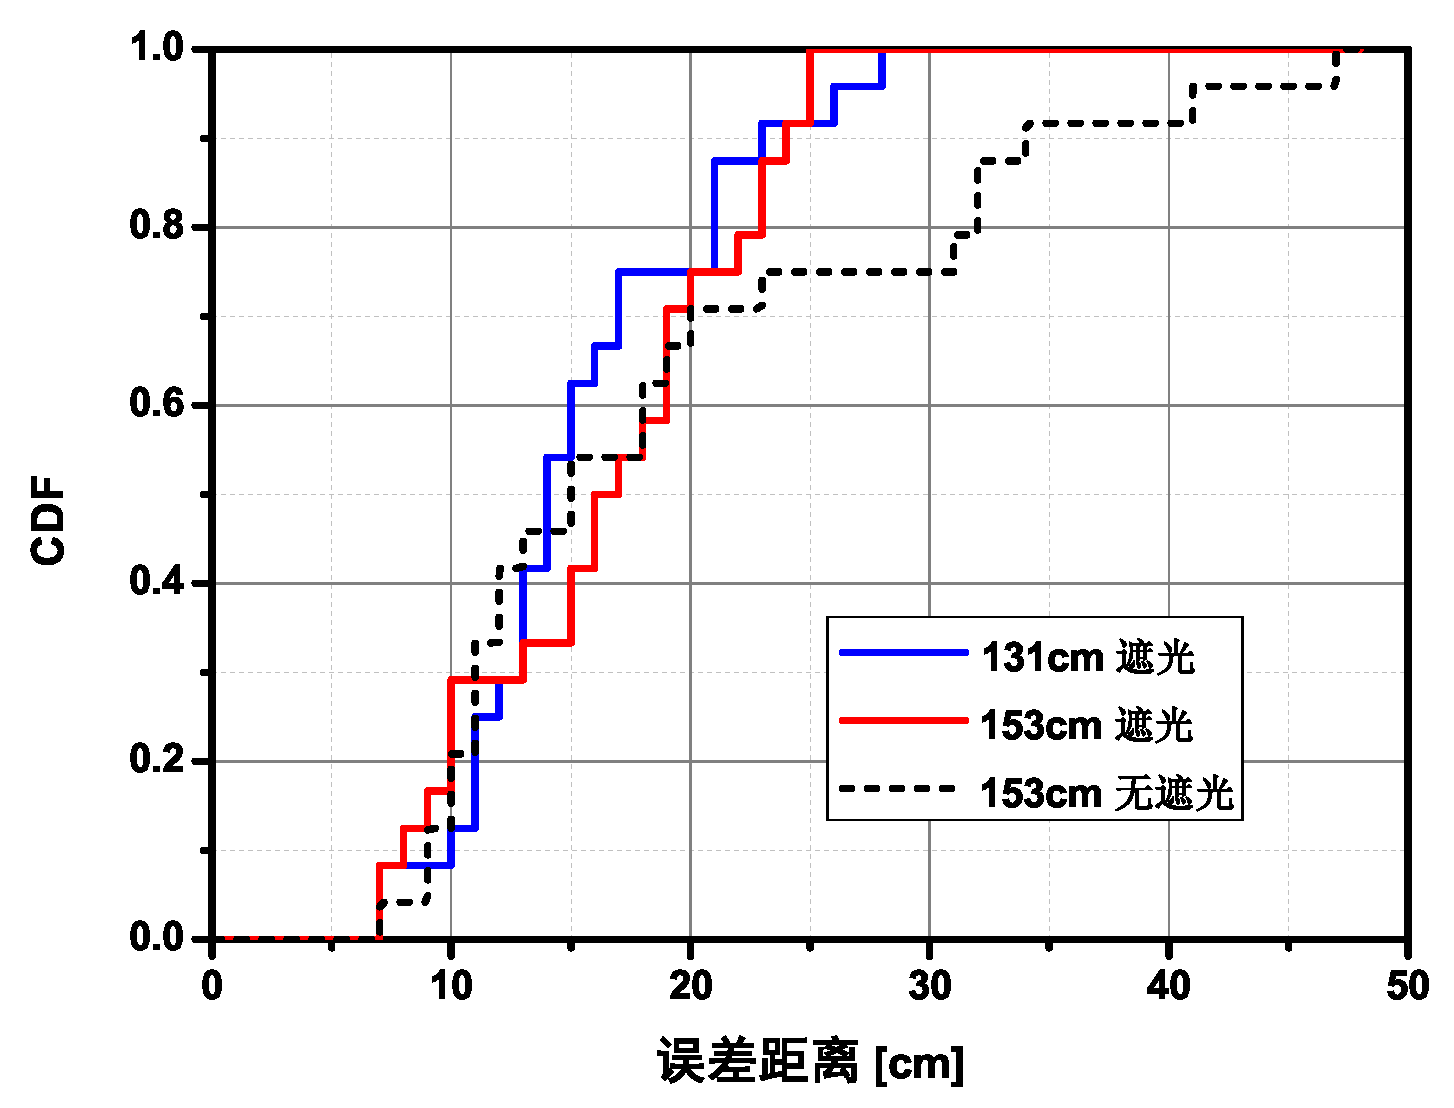
\includegraphics[width=0.7\linewidth]{FIG/5-10.eps}
                \caption{不同条件下的CDF对比}
                \label{fig:cdf}
 \end{figure}

接下来,系统确定了三种情况误差的累积分布函数(Cumulative Distribution Function, CDF),如图 \ref{fig:cdf} 所示。在没有环境光的情况下,CDF曲线几乎相同,而在有环境光的情况下则不是这样,说明环境光比距离的增加对系统性能影响更大。注意,在没有环境光干扰的情况下,所提出的系统可以实现在置信度90$\%$的情况下精度小于22 cm的3D定位,而在有环境光的情况下,这一数字增加到34 cm。显然,系统误差的最大值增加了很多,大于45 cm,反映了在环境光干扰下系统性能严重衰减。

表 \ref{tab:VLP systems} 显示了VLP最新的研究成果。与文献 \parencite{vlp-yang2019visible} 报道的唯一一项NLOS IS-VLP系统研究结果相比,该系统在置信度为90$\%$下的精度为75 cm,很难达到IPS的要求,此外,该系统还需要IMU的辅助。因此,本文所提出的系统更简单、更准确。此外,本文还利用LDM模型计算了反射光产生的IS亮度,为亮度提供了直观的数学表达式。

与LOS VLP相比,所提出的系统克服了LOS链路阴影或遮挡带来的挑战。同时,在仅需要单个IS和LED基础上,通过两个虚拟LED设计实现性能提升。然而,与表 \ref{tab:VLP systems} 中文献 \parencite{vlcp-jin2022adaptive} 和文献 \parencite{vlp-bai2021computer} 的LOS VLP系统相比,所提出的系统性能较差。这是因为硬件系统过于简单和NLOS链路的影响,所提出的NLOS IS-VLP定位精度有限。此外,所提出的3D NLOS IS-VLP算法必须要求相机总是可以捕捉到两个高亮点,由于其中一个是由LED在地板上的投影点形成的,由于LED是固定的,所以它的位置也是固定的。因此,LED在地板上的投影点必须始终在相机的视野内,这大大限制了系统可用的定位范围。考虑到所提出系统性能和定位范围有限,本系统未来还需要进一步改进和优化。
\begin{table}[!t]
                \centering  
                \caption{不同方案的性能比较}  
                \label{tab:VLP systems}  
                \begin{tabular}{lccccc}  
                  \toprule 
                \makebox[0.1\linewidth][l]{$\textbf{方案}$} &\makebox[0.1\linewidth][c]{$\textbf{LED数量}$}&\makebox[0.15\linewidth][c]{$\textbf{接收端类型}$}&\makebox[0.1\linewidth][c]{$\textbf{信道}$}&\makebox[0.2\linewidth][c]{$\textbf{90$\%$置信度的精度}$}&\makebox[0.15\linewidth][c]{$\textbf{辅助传感器}$}\\ 
                \midrule  
                  \parencite{vlcp-jin2022adaptive}&1&5 PDs&LOS&$<$6 cm&No  \\
                  \parencite{vlp-bai2021computer}&4&1 IS&LOS&$<$4.6 cm&No  \\
                  \parencite{vlp-yang2019visible}&1&1 IS&NLOS&75 cm&Yes  \\
                  Ours&1&1 IS&NLOS&$<$22 cm&No  \\
                  \bottomrule 
                \end{tabular}
\end{table}



\section{本章小结}
 本章主要介绍了基于亮度分布模型NLOS IS-VLP系统的基本原理和工作流程以及最后的性能测试。首先,本章提出了一种亮度分布模型,它可以用来表示一次反射光在图像传感器上的亮度分布情况。利用这种亮度分布模型,可以证明在仅有一个LED时,图像传感器上捕捉到的两个高光点可以被视为是两个虚拟的LED通过LOS在图像传感器上面的投影。其中,这两个虚拟LED的位置被证明是LED在反射面的投影和关于反射面的对称点。在通过第三章的NLOS OCC系统得到LED的坐标和高光点的像素坐标之后,可以构建基于两个虚拟LED的LOS IS-VLP系统,利用第二章给出的基于计算机视觉的重投影误差最小化算法实现的接收端的位置估计。从结果可以得知所提出的NLOS IS-VLP系统方案在只有一个LED的情况下能够利用反射光实现3D VLP,成功的克服了本文开篇提出的VLP系统面临的两个主要难点。但是,从系统的定位精度来看,通过反射光进行NLOS IS-VLP的性能还有待提高。